% additional use of \usepackage{beamerthemesplit}
\documentclass{beamer}
\usepackage{beamerthemesplit} % new 
\usepackage{hyperref}
\usepackage{multimedia}
\usepackage[spanish]{babel}
\usetheme{Montpellier}
\usecolortheme{whale}
\definecolor{verde}{rgb}{0,0,1}
\definecolor{rojo}{rgb}{1,0,0}
\definecolor{vio}{rgb}{0.5,0,0.5}
\definecolor{rosa}{rgb}{0.8,0.1,0.1}
\newcommand{\director}{Directores:\\ Mariano Dominguez \& Dante Paz}

\begin{document}
\title{Construction of a catalog of galaxy clusters in collision process.} 
\author{Mart\'in de los Rios, Mariano Dominguez \& Dante Paz}

\frame{\titlepage

%\director
} 

\frame{
\tableofcontents} 

\frame{
\begin{figure}[h!]
 \centering
 \includegraphics[scale=0.3]{./resu.pdf}
 % resu.pdf: 794x595 pixel, 72dpi, 28.01x20.99 cm, bb=0 0 794 595
\end{figure}

}

\section{Mock Catalog.}

\frame{
\tableofcontents[ 
    currentsection, 
    hideothersections, 
    sectionstyle=show/hide, 
    sectionstyle=show/shaded, 
    ] 
}

\subsection{Millenium}

\frame{\frametitle{Millenium Simulation}
\begin{columns}
 \begin{column}{5cm}
\begin{itemize}
 \item $N_{p}=2160^{3} $ \pause
  \item $L=500 Mpc$ \pause
 \item $m_{p}=8.61*10^{8} M_{\odot}$ \pause
 \item $\Omega_{m}=0.25$ ${\color{verde} 0.27 }$ 
 \item $\Omega_{b}=0.045$ ${\color{verde} 0.046 }$ 
 \item $\Omega_{\Lambda}=0.75$ ${\color{verde} 0.75 }$
 \item $h=0.73$ $ {\color{verde} 0.72 }$ 
 \item $n_{s}=1$ ${\color{verde} 0.99 }$ 
 \item $\sigma_{8}=0.9$ ${\color{verde} 0.9 }$ \pause
 \item $Snapshots=64$
\end{itemize}
 \end{column}
 \begin{column}{5cm}
  \begin{itemize}
   \item Millenium simulation: \textit{Springel et al. 2005}.
   \item {\color{verde} WMAP results: \textit{Spergel et al. 2003}}.
  \end{itemize}

 \end{column}

\end{columns}
}

\frame{\frametitle{Study of the merger trees.}
\begin{itemize}
 \item Based on the subhalos merger trees, we construct the merger tree for every fof group in the simulation.
\end{itemize}

\begin{figure}[h!]
 \centering
 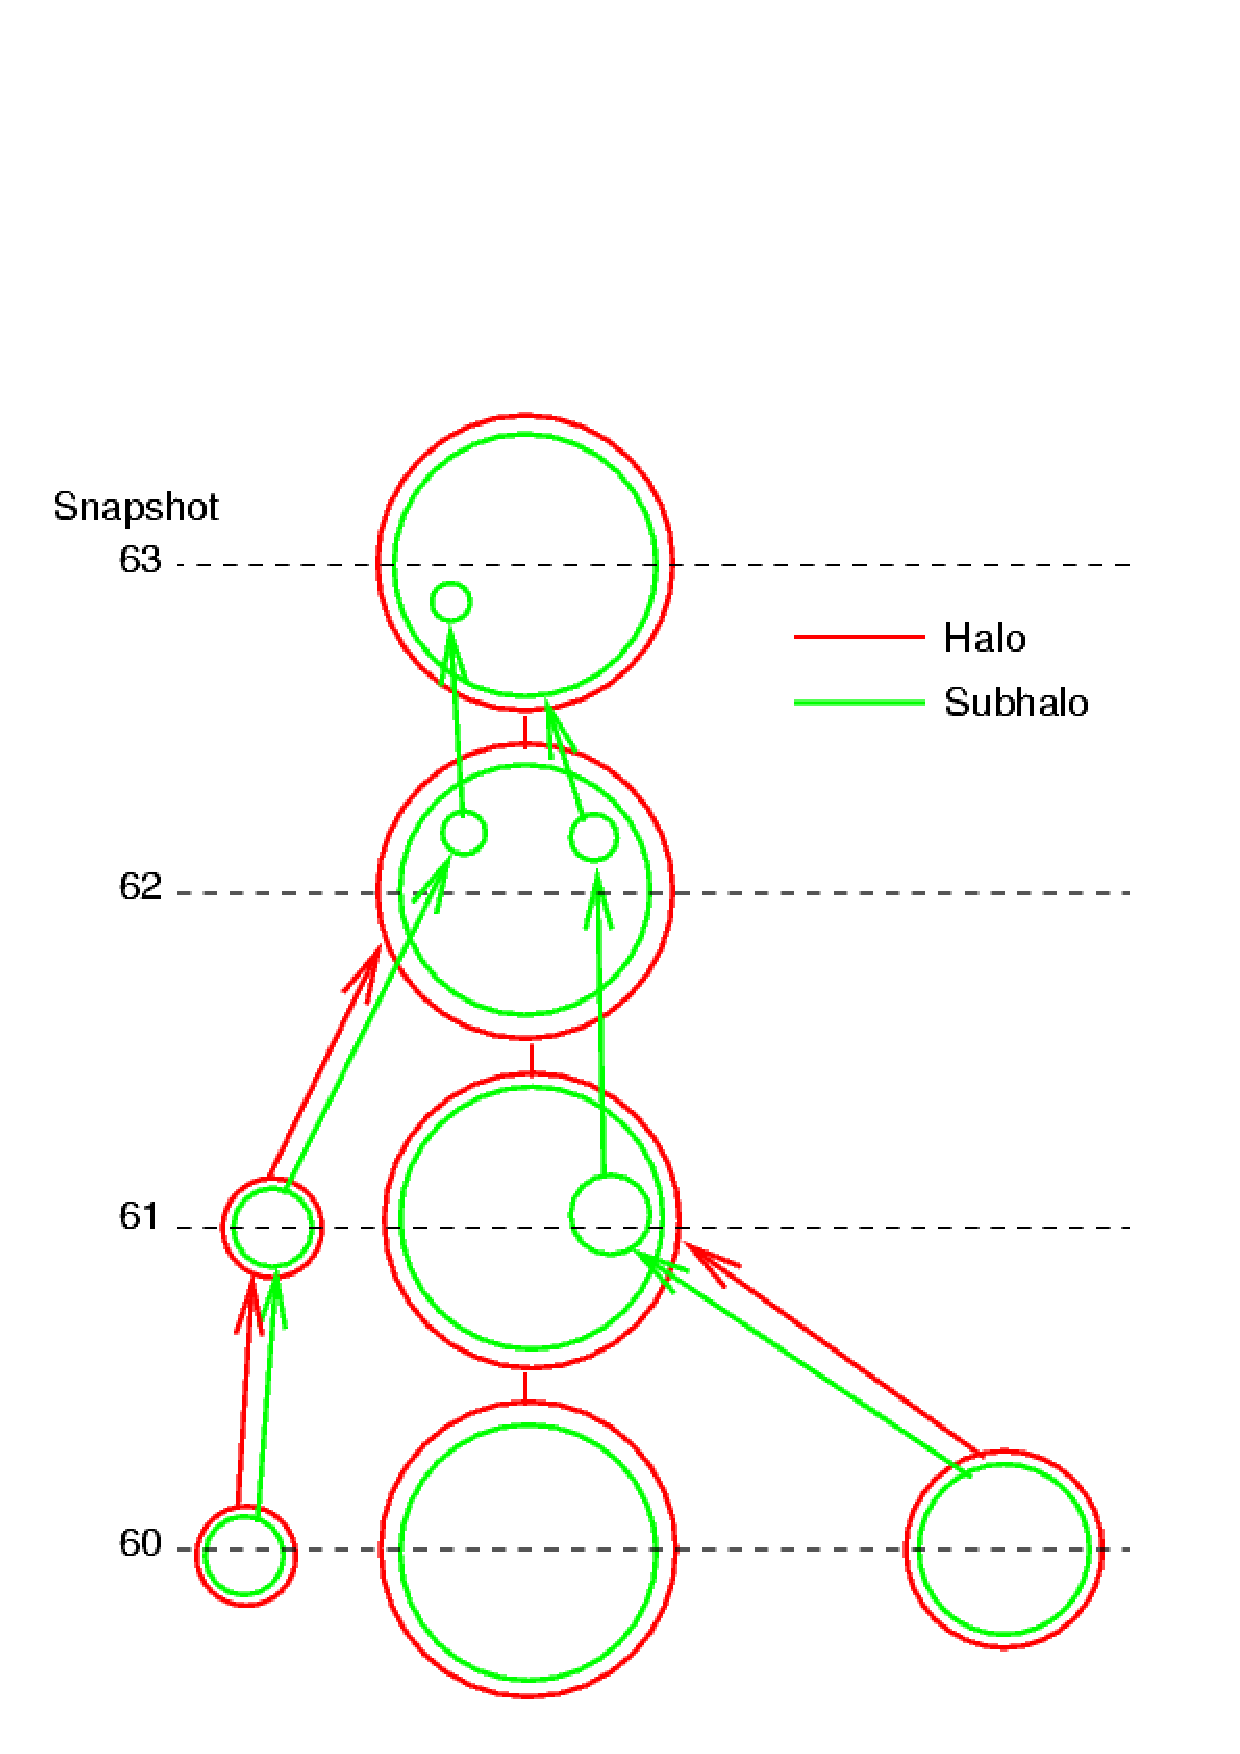
\includegraphics[scale=0.32]{./tree.png}
 % tree.eps: 0x0 pixel, 300dpi, 0.00x0.00 cm, bb=14 14 554 655
\end{figure}

}

%\frame{
%\frametitle{Comparison between mock and real galaxy clusters.}
%\begin{columns}
% \begin{column}{4.2cm}
%  \begin{figure}[h!]
% \centering
% \includegraphics[scale=0.38]{./comparacion_red.png}
 % comparacion_red.png: 480x480 pixel, 72dpi, 16.93x16.93 cm, bb=0 0 480 480
%\end{figure}
% \end{column}
% \begin{column}{5cm}
%  \begin{figure}[h!]
% \centering
% \includegraphics[scale=0.55]{./nu.png}
 % comaracion_bandar.png: 480x480 pixel, 72dpi, 16.93x16.93 cm, bb=0 0 480 480
%\end{figure}
% \end{column}
%\end{columns}
%}



\section{Statistical tests for identification of substructures.}
\frame{
\tableofcontents[ 
    currentsection, 
    hideothersections, 
    sectionstyle=show/hide, 
    sectionstyle=show/shaded, 
    ] 
}

\subsection{The Dressler-Shectman test}
\frame{\frametitle{The Dressler-Shectman test.}
\begin{itemize}
 \item We define the statistic: $\delta^{2}=(\frac{11}{\sigma^{2}})[(v_{local}-v)^{2}+(\sigma_{local}-\sigma)^{2}]$
where \pause
 \item $v$: Mean velocity of the cluster. \pause
 \item $v_{local}$: Mean velocity of the 10 nearest galaxies. \pause
 \item $\sigma$: Velocity dispersion of the cluster. \pause
 \item $\sigma_{local}$: Velocity dispersion of the 10 nearest galaxies. \pause
 \item For each cluster we define the statistic $\Delta$: $\Delta=\Sigma\delta$. \pause
 \item \textit{Pinkney et al. 1996} 
  

  \begin{itemize}
 \begin{tiny}
   \item They say that this is the best test known so far for substructure identification.
   \item The test efficiency is lower when the substructures are aligned along the line of sight, and also when the cluster under consideration have less than 30 galaxy members.
 \item They recommend to look for significant values of the skewness moment on radial velocity distribution.
 \item This test can be used to identify fof-group substructures accreted in a major merger event up to 3 Gyr later. This time interval is equivalent to 10 snapshots in the
 simulation.
 \end{tiny}
  \end{itemize}
\end{itemize}
}


\frame{
\begin{itemize}
 \item Is not possible to derived a theoretical distribution for $\Delta$ in order to build a proper hypothesis test for each cluster.
 To overcome this we compare the obtained $\Delta$ for a given cluster with the distribution of $\Delta$
 obtained from a set of Monte Carlo simulations. For each simulation the velocities are shuffled among the positions.\pause
 \item We define the p-value as
 
 \begin{equation}
  p=\frac{N(\Delta_{MC}> \Delta)}{N_{MC}}
 \end{equation}

\end{itemize}


}

\subsection{Iterative Dressler-Shectman test.}
\frame{\frametitle{Iterative Dressler-Shectman test.} 
Algorithm steps
\begin{itemize}
 \item $\delta^{2}=(\frac{0.2*ngal}{\sigma^{2}})[(v_{local}-v)^{2}+(\sigma_{local}-\sigma)^{2}]$ \pause
 \item We eliminate galaxies with $\delta<0.7 \bar{\delta}$ \pause
 \item We recalculate $\delta^{2}=(\frac{0.2*ngal}{\sigma^{2}})[(v_{local}-v)^{2}+(\sigma_{local}-\sigma)^{2}]$ \pause
 \item The algorithm converges if the number of galaxies between 2 steps is the same.
\end{itemize}
}
%\frame{
%\begin{figure}[h!]
% \centering
% \includegraphics[scale=0.27]{./dlr11.png}
% \includegraphics[scale=0.27]{./dlr21.png}
% \end{figure}
 
% \begin{figure}
% \centering 
%  \includegraphics[scale=0.27]{./dlr31.png}
% \includegraphics[scale=0.27]{./dlr41.png}
 % dlr1.png: 480x480 pixel, 72dpi, 16.93x16.93 cm, bb=0 0 480 480

%\end{figure}

%}



\subsection{Gaussian mixture..}
\frame{\frametitle{Gaussian mixture. (\textit{Mclust})}
The application of the DS test give us a group of galaxies with high probability to lie in a substructure. 
Then, in order to define substructures we identify
clumps of galaxies based on their proximity.

\begin{figure}[h!]
 \centering
 \includegraphics[scale=0.28]{./mclust_class.png}
 \includegraphics[scale=0.28]{./mclust_13.png}
 \includegraphics[scale=0.28]{./mclust_23.png}
 % mclust_class.png: 480x480 pixel, 96dpi, 12.70x12.70 cm, bb=0 0 360 360

\end{figure}

}


\frame{\frametitle{Application of the DS Test in the mock catalog.}
\begin{itemize}
\item We apply the DS test to 2854 clusters with masses higher than $10^{13} M_{\odot}$ and with more than 30 galaxies. \pause
\item We find that 1448 clusters have substructure ($p<0.15$). \pause
\item If we consider only the clusters whose radial velocity skewness is significantly different from zero, the sample is reduce to 715 clusters.
\end{itemize}
}
\frame{
\begin{figure}[h!]
 \centering
 % \includegraphics[scale=0.4]{./histdeltas.png}
 % hist.deltas4pi.png: 480x480 pixel, 72dpi, 16.93x16.93 cm, bb=0 0 480 480
 \includegraphics[scale=0.6]{./hist_snap1.png}


\end{figure}

}
\frame{\frametitle{Application of the iterative DS test to the mock catalog.}
\begin{itemize}
\item We apply the iterative DS test to the sample of 2854 clusters and we find that in 119 the test converges. \pause
\item Over those 119, only 46 clusters have been detected for the traditional DS test complemented with the skewness test.
\end{itemize}

\begin{figure}[h!]
 \centering
 \includegraphics[scale=0.35]{./hist_snap_todo.png}

\end{figure}

}


\frame{\frametitle{Application of gaussian mixture.}
\begin{itemize}
\item We employ the R package Mclust in order to apply gaussian mixture model to the spatial distribution
of galaxies with $\delta >2$. \pause
\item We fits two gaussians to the distribution of galaxies.
\item We find two substructures per cluster in 636 of 715 clusters. \pause
 \item We find two substructures per cluster in 44 of 46 clusters identified for both DS test and the skewness test. \pause
\end{itemize}

}

\frame{
\begin{itemize}
\item 190 clusters of the sample of 715 clusters, have a relative occupation higher than 0.5. \pause
 \item Over the sample of 46 clusters, 20 systems have a relative occupation higher than 0.5.
\end{itemize}

\begin{figure}[h!]
 \centering
 \includegraphics[scale=0.4]{./hist_snap_mclust_dsiter.png}
 \includegraphics[scale=0.4]{./hist_snap_mclust_ds.png}

\end{figure}
}

\frame{\frametitle{Study of the identified substructures.}
\begin{tiny}
 

\begin{itemize}
\item After the substructure identification, each one was related with the subhalo in the mock that have more galaxies in the group identified by
mclust. \pause
\item To improve the identification of the substructure, we calculate the coordinates of the center taking in account the luminosity. \pause
\item After that, we estimate the velocity dispersion and the virial radius.
 
\begin{eqnarray} \label{rvir_disp}
 R_{vir} & = & \frac{\pi}{2} \frac{ngal(ngal-1)}{\sum_{i>j}^{ngal}R_{ij}^{-1}} \nonumber\\
 \sigma &=& \frac{\sqrt{\pi}}{ngal(ngal-1)} \sum_{i=1}^{ngal-1} \omega_{i} g_{i} \nonumber\\
 \omega_{i} &=& i(ngal-i) \nonumber\\
 g_{i} &=& v_{i+1}-v_{i} \nonumber\\ 
\end{eqnarray}
\end{itemize}
\end{tiny}
}

\frame{\frametitle{Study of the identified substructures.}
%\begin{tiny}
 

\begin{itemize}
\item We compare the center of the identified groups with the centers of the associated subhalos, finding a good estimation. \pause
\item We compare the virial radius of the identified groups with the virial radius of the subhalos, finding that we are overestimating the real values. \pause
 \item We compare the velocity dispersion of the identified groups with the velocity dispersion of the associated subhalos, finding that our values are
 in good concordance with the real values. 

\end{itemize}

}

%\frame{

%\begin{columns}
% \begin{column}{5cm}
%\begin{figure}[h!]
% \centering
% \includegraphics[scale=0.35]{./histo_dist_gal_centro.png}
%\end{figure}
% \end{column}
% \begin{column}{5cm}

%\begin{figure}[h!]
% \centering
%  \includegraphics[scale=0.35]{./histo_distvel_gal_centro.png}
%\end{figure}
% \end{column}
%\end{columns}
%}

%\frame{
%\begin{itemize}
%\item We will consider members of a group, only that galaxies that have a projected distances lower than the virial radius and
%with a difference of radial velocity lower than two times the velocity dispersion.

%\end{itemize}
%\begin{figure}[h!]
% \centering
% \includegraphics[scale=0.32]{./puto.png}
%\end{figure}
%}

\frame{

With this association between groups and subhalos in the mock, we find 3 cases:

\begin{enumerate}
\item Clusters where we identify the type 0 subhalo (the principal subhalo of the fof group) and a type 1 subhalo. \pause
\item Clusters where we identify two type 1 subhalos. \pause
 \item Clusters where Mclust find two substructures that are associated to the same type 0 subhalo. \pause
\end{enumerate}

Of the 715 clusters, we find 28 with 2 substructures with a relative occupation higher than $0.5$ while each group have more than 3
galaxy members. From this 28, in 19 we find the type 0 subhalo and a type 1 subhalo (case 1), in 4 we find 2 type 1 subhalos (case 2) 
and in 5 we identify a false substructure (case 3).

}

%\frame{
%\begin{figure}[h!]
% \centering
% \includegraphics[scale=0.34]{./histo_arribo.png}
% \includegraphics[scale=0.34]{./histo_masarel_mock.png}

%\end{figure}

%}



%------------------------------------------------------------------------------------------------------------------------------------------------
%------------------------------------------------------------------------------------------------------------------------------------------------
%------------------------------------------------------------------------------------------------------------------------------------------------
%------------------------------------------------------------------------------------------------------------------------------------------------
%------------------------------------------------------------------------------------------------------------------------------------------------
%------------------------------------------------------------------------------------------------------------------------------------------------
%------------------------------------------------------------------------------------------------------------------------------------------------
\section{Results.}
\frame{
\tableofcontents[ 
    currentsection, 
    hideothersections, 
    sectionstyle=show/hide, 
    sectionstyle=show/shaded, 
    ] 
}

\subsection{Real catalogs of galaxy clusters.}
\frame{\frametitle{Application of the method of detection to real catalogs.}
\begin{small}
 

 \begin{center}
\begin{tabular}{||l|l|l|l|l||}
\hline
Catalog & Berlind et al. & Tempel et al. & Eke et al. & Mock\\
\hline
Galaxy survey & SDSS DR3 & SDSS DR8 & 2dF & -\\
\hline
$N^{\circ}$ galaxy clusters & $8148$ & $77858$ & $28877$ & -\\
\hline
$N^{\circ} clusters (N_{gal}>30)$ & $77$ & $389$ & $144$  & $2854$\\
\hline
$pval > 0.15$ & $30$ & $246$ & $112$ & $1448$\\
\hline
$pval > 0.15+SK$ & $30$ & $132$ & $60$ & $715$\\
\hline
Ds iter & $20$ & $86$ & $41$ & $46$\\
\hline
Mclust & $15$ & $80$ & $38$ & $44$\\
\hline
\end{tabular}
 \end{center}
\end{small}

}
%------------------------------------------------------------------------------------------------------------------------------------------------
%------------------------------------------------------------------------------------------------------------------------------------------------
%------------------------------------------------------------------------------------------------------------------------------------------------
%------------------------------------------------------------------------------------------------------------------------------------------------
%------------------------------------------------------------------------------------------------------------------------------------------------
%------------------------------------------------------------------------------------------------------------------------------------------------
%------------------------------------------------------------------------------------------------------------------------------------------------

\section{Future work.}
\frame{
\tableofcontents[ 
    currentsection, 
    hideothersections, 
    sectionstyle=show/hide, 
    sectionstyle=show/shaded, 
    ] 
}

%\frame{
%\frametitle{Summary.}
%\begin{itemize}
%\item We constructed a mock catalog of galaxies. \pause
%\item We construct a merger tree for the fof groups. \pause
%\item We study different methods of substructure identification. \pause
%\item We study the merger trees of the clusters identified by the different methods. \pause
%\item We identify and study the substructures of the clusters, finding the galaxies who lives in the substructure and calculating
%some of its fundamental properties. \pause
%\item We apply the methods to real galaxy surveys. \pause
%\item We construct a catalog of galaxy clusters that are in a collision process.
%\end{itemize}
%}

\frame{\frametitle{Future work.}
\begin{itemize}
\item Improve our identification methods (Make the mock catalog more similar to sloan, elaborate new methods of substructure identification, etc.). \pause
 \item Calibrate the method with light cone mock catalogs, in order to apply this to more deep real catalogs. \pause
 \item Study the physics properties of the galaxies that belong to the identify substructures. \pause
\item Perform astrophysical test over our sample of colliding cluster candidates of the catalog looking for
impose some constraints on dark matter particle properties.
\end{itemize}


}

\begin{frame}[plain]
\begin{figure}[h!]
 \centering
 \includegraphics[scale=0.4]{./gracias.pdf}
 % gracias.png: 657x518 pixel, 72dpi, 23.18x18.27 cm, bb=0 0 657 518
\end{figure}
\end{frame}
\end{document}

